\documentclass[11pt, a4paper]{article}
\usepackage[left=25mm,right=15mm,top=15mm,bottom=15mm]{geometry}
\usepackage[utf8x]{inputenc}
\usepackage[L7x]{fontenc}
\usepackage[lithuanian]{babel}
\usepackage{url}
\usepackage{float}
\usepackage{graphicx}
\usepackage{amsmath}
\usepackage{fancyhdr}
\usepackage{datetime}
\graphicspath{{img/}}
\usepackage{tikz}
\usepackage{gensymb}
\usepackage{subfig}
\usetikzlibrary{arrows}

\begin{document}

  \begin{titlepage}
    \begin{center}
      \textsc{\LARGE Vilniaus Gedimino Technikos universitetas}\\[2mm]
      \textsc{\Large Elektroninių sistemų katedra}\\[70mm]
      \textsc{\Large Objekto padėties nustatymas taikant MEMS jutiklius}\\[60mm]
      \textsc{\Large Juodraštis}\\
      {\large \today  \ \currenttime}\\
      \vfill
      {\large Vilnius \\ \the\year}
    \end{center}
  \end{titlepage}

  \section{Įvadas}

  Objekto padėties nustatymas turi dvi plačias pritaikymo sritis: inercinė navigacinė ir žmogaus judesio sekimo sistema \cite{schlomer2008gesture};

Objekto pozicijos nustatymas, panaudojus inercinius jutiklius remiasi prielaida, jog objektas lieka ramybės būsenoje tol, kol jį nepaveikia išorinė jėga. Tokia jėga suteikia objektui pagreitį. Jeigu rasta pagreitį galima išmatuoti ir suintegruoti, pagreičio ir pozicijos kitimas gali būti išmatuoti. Reikia nepamiršti, kad tokiu atveju matavimą sudarys dvi komponentės -- pagreitis dėl gravitacijos ir išorinės veikiančios jėgos pagreitis. Norint pašalinti gravitacijos komponentę iš pagreičio matavimo, reikia žinoti kokiu kampu akcelerometras yra vertikalės atžvilgiu.
Tokio kampo matavimui, reikalingas kitas jutiklis, kuris vadinasi giroskopas. Jis matuoja kampo greitį, kurį matematiškai integruojant, galima rasti kampo greičio pokytį nuo pradinio, žinomo kampo \cite{sukkarieh2000low}.

Akcelerometras suteikia pagreičio matavimą norimam objektui. Dažniausiai tokie matavimai yra užrašomi $x$, judėjimą tiesiai, $y$, šonu ir $z$ vertikaliai. Giroskopas suteikia matavimus, kurie dengia nurodytas ašis ir yra užrašomi $\theta$, sūkiui, $\beta$ polinkiui ir $\gamma$ vingiavimui, kaip pavaizduota \ref{tikz:axis_of_the_system} pavyzdyje. Tokių inercinių įverčių naudojimas turi pagrindinį privalumą -- stebimo objekto polinkis ir pagreitis gali būti vertinami bet kokioje navigacijoje.  

\begin{figure}[H]
    \centering
    \caption{Objekto pozicijos pagreičio pokyčio ašys, $x$, $y$ ir $z$. Sūkio matmenys apie ašis $\theta$, $\beta$ ir $\gamma$.}
    \label{tikz:axis_of_the_system}
    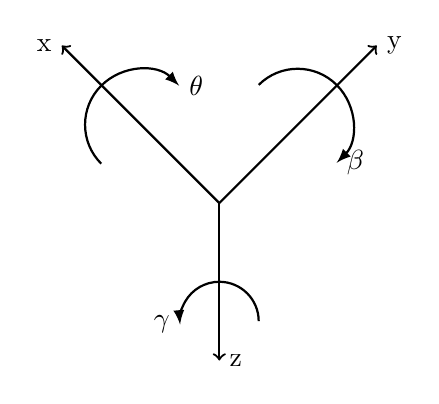
\begin{tikzpicture}
        % axis
        \draw[thick, black, ->] (0,0) -- ( 2, 2) node [right] {y};
        \draw[thick, black, ->] (0,0) -- (-2, 2) node [left] {x}; 
        \draw[thick, black, ->] (0,0) -- ( 0,-2) node [right] {z};
        % arc
        \draw[thick, -latex] ( 0.5,  1.5) arc (135:-45:0.70) node [right] {$\beta$}; 
        \draw[thick, -latex] (-1.5,  0.5) arc (225:45:0.70) node [right] {$\theta$};
        \draw[thick, -latex] ( 0.5, -1.5) arc (0:185:0.5) node [left] {$\gamma$};
    \end{tikzpicture}
\end{figure}

Inercinės navigacijos sistemos yra naudojamos labai plačiai lėktuvuose, raketose, kosmoso laivuose, povandeniniuose ir vandens laivuose \cite{woodman2007introduction}. Progresas gaminant MEMS įrenginius, sudarė galimybes kurti mažas ir lengvas navigacines sistemas. Tokie privalumai leidžia praplatinti įrenginių panaudojimo galimybes ir šiuo metu įtraukia tokias sritis kaip žmogaus ir gyvūnų judesio sekimą.

Tačiau reikia nepamiršti ir apie klaidas, kurias sukelia nuolatinė dedamoji, santykio įverčiai ir nelinijines sistemos įtakos jutiklio verčių nuskaitymo metu. Tokios klaidos yra pagrindinė priežastis atsirasti netikslumams navigacinėje sistemoje per laiko vienetą. Netikslumai sąlygoja akselerometro įverčius, kuriuos tampa labai sunku atskirti tarp gravitacinio lauko ir objekto judėjimo, ko pasekoje objekto pozicijos matavimas toliau yra dar netikslesnis. Kadangi inerciniai jutikliai yra tokio tipo, kuriems yra labai svarbi tiksli prieš tai buvusi pozicija, bet kokia klaida skaičiuojant prieš tai buvusia pozicija, įtakoja ir dabartinės pozicijos skaičiavimą. Tokiu būdu, su laiku navigacinė sistema tampa visiškai netiksli ir praranda visą savo vertę.

  \section{MEMS jutikliai}

  Šiame skyriuje apžvelgti MEMS pagreičio ir giroskopo tipo jutikliai. 
Aptariama, kokie yra didžiausi jų privalumai ir trūkumai (didelis duomenų triukšmas ir būdai jiems kompensuoti ar mažinti).

\subsection{Giroskopas}

MEMS tipo jutiklis \cite{perlmutter2012high} yra gaminamas staklėmis iš silikono mikro-apdorojimo būdu, turi labai mažai dalių, o jo gamybos kaštai yra gana maži.

MEMS giroskopai yra veikiami \textit{Coriolio efekto}, kuris sako, jog turint koordinačių ašį, sukantis kampiniu greičiu $w$, objektas su mase $m$, kuris juda greičiu $v$, yra veikiamas jėgos

\begin{equation}
    F_c = -2m(w \times v)
\end{equation}

MEMS giroskopai susideda iš vibracinės kilmės elementų, kurie yra naudojami matuojant \textit{Coriolio} efektą. 
Egzistuoja labai daug vibracinių geometrijų, tarp kurių yra vibracinis ratas ir kamertono giroskopai. 
Paprasčiausia geometrija susideda iš vienos masės, kuri skirta vibruoti viena ašimi. 
Kai tik giroskopas yra pasukamas, įvedama antrinė vibracija statmenai pirminei ašiai dėl \textit{Coriolis} jėgos. 
Dėl to, kampinis greitis gali būti apskaičiuojamas, matuojant antrinį apsisukimą. 
Šiuo metu MEMS jutikliai negali pasiekti tokio tikslumo lygio, kokį siūlo optiniai jutikliai, tačiau yra tikimasi, kad ateityje MEMS jutikliai tikslumu nebus prastesni nei optiniai jutikliai.

MEMS jutikliai turi labai daug privalumų, palyginti su kitais jutikliais \cite{titterton2004strapdown}:

\begin{itemize}
    \item mažas dydis;
    \item mažas svoris;
    \item patvari konstrukcija;
    \item mažos galios naudojimas;
    \item labai greitas paleidimo laikas;
    \item pigi gamyba, esant dideliam mastui;
    \item patikimi;
    \item reikalauja labai mažai priežiūros;
    \item gali būti naudojami sudėtingomis sąlygomis;
\end{itemize}

\subsubsection{Nuolatinė dedamoji}

Vidutinis kampo pokyčio matavimas, palaikant visišką giroskopo ramybės būseną, yra laikomas nuolatine giroskopo dedamąja. 
Matuojama yra $\degree/h$. 
Nuolatinės dedamosios klaida $\epsilon$ yra apskaičiuojama integruojant ir priklauso nuo laiko $\theta(t) = \epsilon \cdot t$.

Klaida gali būti nustatyta, panaudojus labai ilgo laikotarpio vidutinę vertę, kuomet giroskopas yra paliktas visiškos ramybės būsenos ir nėra veikiamas jokių išorinių jėgų. 
Kai tik nuolatinė dedamoji yra žinoma, labai yra svarbu ją kompensuoti tikro matavimo metu.

\subsubsection{Atsitiktinis kampinis pokytis}

Jutiklio vertės matavimo metu yra galimas triukšmas, sukeliamas terminių ir mechaninių trukdžių, kurių dažnis yra žymiai didesnis už jutiklio vertės matavimo dažnį.
Tokių veiksnių rezultatas yra signalas, kuriame yra balto triukšmo. 
Tai yra paprasčiausia eilė skaičių, kurių vidurkis lygus nuliui.
Nėra jokios koreliacijos ir yra visiškai atsitiktiniai skaičiai. 
Tokiu būdu kiekvienas atsitiktinis skaičius yra tolygiai paskirstytas ir turi baigtinį $\sigma^2$ pasiskirstymą.

Net ir neišvedus formulės (detalus išvedimas yra pateikiamas \cite{woodman2007introduction}) galima teigti, jog triukšmas įveda ,,atsitiktinio vaikščiojimo'' (angl. \textit{random walk}) klaidą integraliniame signale, kuri yra nulinio vidurkio ir kurios variacija didėja nuo laiko pokyčio šaknies.
\begin{equation}
    \sigma_{\theta} (t) = \sigma \cdot \sqrt{ \delta t \cdot t}
\end{equation}
Čia $\sigma$ yra triukšmo signalo pokytis, $t$ yra visas jutiklio įverčio nuskaitymo periodas, o $\delta t$ yra laiko skirtumas tarp nuskaitymų.

Kadangi dominantis įvertis yra kaip triukšmas, lemiantis integralinį signalą, labai dažnai gamintojai nurodo gaminamo jutiklio atsitiktinį kampinį pokytį. Jis yra žymimas $\degree/\sqrt{h}$. 
Pavyzdžiui, jeigu jutiklis yra $0,3\degree / \sqrt{h}$, tai reiškia, jog po vienos valandos standartinės variacijos pozicijos orientacijos klaida sudarys $0,3\degree$, po dviejų valandų $\sqrt{2} * 0,3 = 0.42 \degree$.

\subsection{Nuolatinės dedamosios stabilumas}

Nuolatinė dedamoji MEMS giroskope keičiasi laikui bėgant dėl virpėjimo triukšmo elektronikos ir kituose įtaisuose, kurie potencialiai gali būti paveikti atsitiktinio virpėjimo. 
Virpėjimo triukšmas yra $1/f$ spektro, kurio efektai yra pastebimi elektroniniuose komponentuose, esant žemiems dažniams. 
Esant aukštiems dažniams virpėjimas yra uždengiamas balto triukšmo. 
Nuolatinės dedamosios nestabilumas, kuris kyla dėl virpėjimo, dažniausiai yra modeliuojamas kaip atsitiktinis kampinis pokytis.

Nuolatinės dedamosios stabilumo įvertis nurodo, kiek gali keistis per fiksuotą laiko tarpą. 
Dažniausiai imamas $100~s$ laiko rėžis, kuomet aplinka visiškai nesikeičia. 
Įvertis žymimas kaip $1\sigma$ ir matuojamas $\degree/h$ arba $\degree/s$, kai įranga yra labai netiksli. 
Nuolatinės dedamosios stabilumas yra modeliuojamas atsitiktinio vaikščiojimo procesu. 
Tai galima interpretuoti turint $B_t$ kaip dedamosios vertė laiku $t$, tuomet $1\sigma$ stabilumas $0,01\degree/h$ per 100 sekundžių reiškia, kad dedamoji laiku $t+100$ yra atsitiktinis skaičius, kurio vertė yra tikėtina $B_t$ su $0,01\degree/h$ variacija. 
Po tam tikro laiko, variacija sukuria atsitiktinį vaikščiojimą, kurio nuokrypis didėja per laiko vieneto šaknį. 
Dėl šitos priežasties nuolatinės dedamosios stabilumas yra žymimas kaip dedamosios atsitiktinis vaikščiojimo matas

\begin{equation}
    BRW (\degree / \sqrt{h}) = \frac{BS(\degree/h)}{\sqrt{t(h)}},
\end{equation}
kur $t$ yra nuolatinės dedamosios stabilumo laikas.

Praktikoje yra truputį kitaip. 
Jeigu stabilumas būtų modeliuojamas kaip atsitiktinis vaikščiojimas, tai integracinis įverčio skaičiavimas smarkiai padidintų klaidos įvertį. 
Dėl to, yra nutarta nustatyti rėžius, kuriuose yra nurodomas stabilumas.

\subsubsection{Temperatūros efektai}

Temperatūros svyravimai kyla dėl aplinkos temperatūros nepastovumo ir pačio jutiklio temperatūros nepastovumo. 
Tokie svyravimai natūraliai įtakoja ir nuolatinę dedamąja. 
Jie visiškai nėra nurodomi nuolatinės dedamosios klaidos skaičiavimuose.

Bet koks likutinis nuolatinės dedamosios įterpimas dėl temperatūros pokyčio smarkiai padidins įverčio klaidą ir klaida laikui bėgant didės.
Santykis MEMS jutikliuose tarp temperatūros ir klaidos yra netiesinis.
Dauguma inercinių matavimo sistemų turi savo viduje temperatūros daviklį, todėl matavimo klaidą galima kompensuoti tokiu būdu. 
Kai kurios matavimo sistemos siūlo automatinį klaidos taisymą.

\subsubsection{Kalibravimo klaidos}

Kalibravimo klaidų terminas susieja grupę klaidų šaltinių, kurie susideda iš santykio faktoriaus, lygiavimo ir giroskopų tiesiškumo. 
Tokio tipo klaidų galima pastebėti tik išoriškai veikiant jutiklį ir stebint nuolatinės dedamosios pokytį. 
Tai sukelia integracinio signalo netikslumų, prie kurių prisideda papildomi svyravimai, kurių dydis yra santykis tarp pokyčio ir vykdymo laiko. 
Dažniausiai tokio tipo klaidas galima išmatuoti ir jas kompensuoti.

% Akcelerometras

\subsection{Pagreičio jutiklis}

Mikro-staklių pagaminti silikoniniai pagreičio jutikliai naudoja tokius pačius principus, kaip ir mechaniniai ar kietieji jutikliai. 
Egzistuoja du pagrindiniai MEMS pagreičio jutiklių tipai. 
Pirmas tipas yra mechaniniai pagreičio jutikliai, kurie yra pagaminti iš silikono. 
Jie veikia lygiai tokiais pačiais principais, kaip ir mechaniniai jutikliai. 
Antras jutiklių tipas - kurie matuoja vibracijos pokyčius vibraciniam elemente, ko pasekoje yra stebimi įtampos pokyčiai.

Pagreičio MEMS jutiklių privalumai yra lygiai tokie patys, kaip ir MEMS giroskopinių jutiklių. 
Taip pat, pagrindinis tokių jutiklių minusas prieš kito gaminimo tipo jutiklius - mažas tikslumas. 

\subsubsection{Nuolatinė dedamoji}

Vertės dedamoji, pagreičio matavimo jutiklyje, yra skirtumas tarp matuojamos vertės ir realios vertės, matuojama $m/s^2$.
Pastovios dedamosios klaida $\epsilon$, po dvigubos integracijos, sukuria klaidą, kuri laikui bėgant didėja keturis kartus. 
Sukaupta klaida, priklausomai nuo pozicijos yra

\begin{equation}
    s(t) = \epsilon \cdot \frac{t^2}{2},
\end{equation}
kur $t$ yra integravimo laikas.

Yra galimybių vertinti dedamąją atliekant matavimus su duotu jutikliu labai ilgą laiką, kuriuo neveikia jokia išorinė jėga. 
Deja, visiškai izoliuoti jutiklio nėra galima, kadangi iškarto erdvėje pradeda veikti gravitacija, kuri veikia jutiklį, patiekdama savo nuolatinę dedamąja. 
To pasekoje, labai svarbu yra žinoti įrenginio pozicija žemės atžvilgiu, iš kurios pusės veikia gravitacinė jėga. Praktikoje tai yra pasiekiama naudojant kalibravimo procedūra, kurios metu įrenginys yra pritvirtinamas prie paviršiaus, kurio orientacija gali būti kontroliuojama labai tiksliai.

\subsubsection{Atsitiktinis pagreičio pokytis}

Pagreičio MEMS jutiklio išėjimo matavimai yra veikiami balto triukšmo. 
Kaip jau buvo paminėta giroskopo atsitiktinio kampo pokyčio poskyryje, balto triukšmo integracija sudaro sąlygas variacijai didėti proporcingai $\sqrt{t}$. 
To pasekoje, jutiklio išėjime yra stebimas atsitiktinis verčių vaikščiojimas, kuris vertinamas $m/s/\sqrt{h}$. Praleidžiant standartinės variacijos išvedimą, kuris yra aprašytas \cite{woodman2007introduction}, galima iškarto teigti, kad pagreičio jutiklio baltas triukšmas sukuria antro lygio atsitiktinį verčių vaikščiojimą pozicijoje, su vidurkiu, kuris lygus nuliui ir standartiniu nuokrypiu

\begin{equation}
    \sigma_{s}(t) \approx \sigma \cdot t^{3/2} \cdot \sqrt{\frac{\delta t}{3}},
\end{equation}
kuris didėja proporcingai nuo $t^{3/2}$. 
Čia $t$ yra visas matavimo laikas, $\delta t$ yra skirtumas tarp įverčio matavimo laikų.

\subsubsection{Vibraciniai triukšmai}

MEMS tipo pagreičio jutikliai yra veikiami vibracijos triukšmo, kuris sukelia nuolatinės dedamosios stabilumo klaidą per laiką. 
Tokie nukrypimai yra dažnai modeliuojami kaip nuolatinės dedamosios atsitiktiniai judėjimai, kaip jau buvo aprašyta giroskopo atveju. 
Naudojantis tokiu modeliu, vibracijos sukuria antro lygio atsitiktinio vaikščiojimo triukšmą pagreičiui, proporcingai $t^{3/2}$ ir trečio lygio atsitiktinį vaikščiojimą, kuris yra proporcingas $t^{5/2}$.

\subsubsection{Temperatūros efektai}

Kaip ir giroskopu atžvilgiu, temperatūros pokyčiai įtakoja vibracinius pokyčius, kas sukelia dedamosios nestabilumus išėjimo signale. 
Dedamosios santykis su temperatūra labai priklauso nuo įrangos, tačiau dažniausiai jis yra ne linijinis. 
Bet koks liekamasis nuolatinės dedamosios komponentas sukelia klaida, kuri didėja keturgubai bėgant laikui. 
Pagreičio jutiklio korekcijos dėl temperatūros kai kurie matavimo įrenginiai automatiškai kompensuoja.

\subsubsection{Kalibravimo klaidos}

Kalibravimo klaidos atsiranda kaip nuolatinės dedamosios klaidos. 
Jie pasirodo įverčiuose tik tuomet, kai jutiklis yra veikiamas kažkokio pagreičio jėgos. 
Taip pat verta stebėti gravitaciją, kadangi ji gali sukelti tokias laikinas klaidas ir tuomet, kai jutiklis yra pastovioje pozicijoje ir nėra veikiamas išorinės pagreičio jėgos.



  \section{Literatūros apžvalga}

  \subsection{Pozicijos nustatymas naudojant mobilų telefoną}

Pirmas darbas apžvalgai yra \cite{willemsenconcept}, ``Concept for building a MEMS based indoor localization system''. Darbas pasiūlo galimos navigacinės sistemos prototipą, kuris remiasi inerciniais jutikliais. Kaip prototipo pagrindą buvo pasirinkit du mobilieji telefonai, kurie turi barometrą, pagreičio ir giroskopo jutiklį.

Darbas pradedamas prototipo pagrindo apžvalga, o konkrečiai nuo barometro. Barometras kaip matavimo įrenginys gali būti panaudotas pastato vidaus navigacijai, kurio pagalba galima nustatyti aukštą, kuriame yra stebimas objektas. Oro slėgis $p_i$ yra konvertuojamas į barometro aukščio formulę

\begin{equation}
    h_i = \Bigg( 1 - \sqrt[\leftroot{-2}\uproot{2}5.255]{ \frac{p_i}{1013.25} } \Bigg) \times \frac{288.15}{0.0065},
\end{equation}

Testavimo bazė buvo panaudotas \textit{HafenCity University} pastatas, kuris turėjo keturis aukštus. Duomenų surinkimo metu, jutiklis buvo perneštas per visus pastato aukštus su 4-3-2-1-1-2-3-4 seka. Rezultatai yra pateikiami \ref{fig:floor_detection_with_barometer_data} pavyzdyje.

\begin{figure}[H]
    \centering
    \includegraphics[width=300px]{img/floor_detection_with_barometer_data.png}
    \caption{Barometro naudojimas aukšto atpažinimui \cite{willemsenconcept}.}
    \label{fig:floor_detection_with_barometer_data}
\end{figure}

Grafike pavaizduotos juodos linijos vaizduoja gryną signalą, žalia juosta žymi vidutinį signalo įvertį per $1~s$ laikotarpį. Rezultatai labai ryškiai parodo, kad barometras gali būti panaudotas aukštui nustatyti.

Toliau yra nagrinėjamas pagreičio jutiklio pritaikymo galimybės. Iškarto yra teigiama, jog dviguba integracija, kuri gali būti panaudota apskaičiuojant nukeliautą atstumą yra visiškai negalimas panaudoti matmuo, kadangi pagreičio jutiklis yra labai linkęs dreifuoti. To pasekoje, jutiklis yra panaudojamas tik kaip žingsnių matuoklis. Žingsniui nustatyti yra panaudojamas sekantis metodas. Pirmiausiai yra laukiama kuomet pagreičio pokyčio vertė įkopia į teigiamą pusę. Tuomet algoritmas laukia neigiamo gradiento signale. Kai tik jis yra randamas -- detektuojamas žingsnis. Taip pat yra panaudojamas verčių buferis (angl. \textit{buffer}), norint minimizuoti klaidingą žingsnio radimą.

Kaip ir bet kokį jutiklį, pagreičio jutiklį reikia kalibruoti, nors iš pirmo žvilgsnio žingsnių atpažinimui to nereikia, tačiau būtent akselerometro pozicija nusako ašių gradientą, todėl norint tiksliai žinoti ašių etaloną, reikalinga kalibravimas. Tam autoriai vietinės srities gravitacijos įverčių duomenų bazę. Kalibravimo metodas yra paremtas \cite{wendel2011integrierte} Kalman filtru. Konteksto funkcija yra įgyvendinama per sferinį Pitagorą:

\begin{equation}
    g^2 = a_{xref}^2 + a_{yref}^2 + a_{zref}^2
\end{equation}

Santykis tarp atspirties (angl. \textit{reference}) vertės ir matavimo vertės, su pataisymu ir papildoma dedamąja yra išreiškiama

\begin{equation}
    a_{xref} = s_x (a_x + b_x)
\end{equation}

\begin{equation}
    a_{yref} = s_y (a_y + b_y)
\end{equation}

\begin{equation}
    a_{zref} = s_z (a_z + b_z)
\end{equation}

Funkcinis modelis gali būti parenkamas taip, jog mastelio $s$ ir dedamosios $b$ parametrai yra atitinkamai pataisomi.

Kalibravimui reikalingi parametrai yra randami pirmiausiai apverčiant prototipinį įrenginį porą kartų aplink savo matavimo ašis. To tikslas yra sujungti pagreičio jutiklio kiekvieną iš teigiamos ir neigiamos ašių su gravitacija. Labai svarbu yra užtikrinti, kad sukimas vyksta lygiai pagal jutiklio centrą, kad išvengti papildomų kalibravimo klaidų.

Sekantis įrenginys nagrinėjimui yra giroskopas ir jo sukimo pokytis. Orientacijos įvertis yra gaunamas paprasčiausiai integruojant sukimo pokytį. Toks integralas sudaro galimybei atsirasti dreifui. Dreifas yra didžiausias klaidos šaltinis pigiuose MEMS jutikliuose. Darbe yra pastebėta, jog kalibruoti giroskopą nėra būtina, bet labai svarbu yra identifikuoti dreifą prieš pradedant matavimus. Tokiu tikslius matavimo pradžioje giroskopas yra paliekamas ramybės būsenoje. Tai yra pasiekiama įrenginį prilaikant ant stalo. Dažniausiai tokiu atveju bus matoma tiesiog nuolatinė dedamoji, tačiau niekas negarantuoja stabilios nuolatinės dedamosios. Klaida gali kisti per laikotarpį, todėl pažymėtina yra atlikti papildomas korekcijas per matavimo laikotarpį.

Toliau yra pateikiamas pavyzdys su naudojama įranga, konkrečiai su Samsung Galaxy Nexus telefonu. Labai svarbi detalė yra automatinė nuolatinės dedamosios korekcija, kuri įrenginyje įvyksta po $8~s$. Tai yra vadina \textit{ZUPT} (angl. \textit{Zero velocity UPdaTe}). Korekcija įvykdoma tik tuomet, kai jutiklis nėra judinamas. 

Pereinama nuo pačių jutiklių duomenų prie duomenų apdorojimo. Jutiklių matmenų nuskaitymui yra panaudojamas kelio skaičiavimo metodas (angl. \textit{Dead Reckoning}). Navigacijos labui, kampo pokytis yra integruojamas, o pagreičio jutiklis yra panaudojamas tik žingsnio radimui. Turint informacijos apie žingsnio ilgį ir esamą kryptį, santykinė pozicija gali būti apibrėžta taikant vektorinę sudėtį (angl. \textit{polar appending}). Įvertinant triukšmą, kuri turi tiek pagreičio, tiek giroskopo jutikliai vien tik jų duomenimis pasikliauti nėra galima, todėl reikia įsivesti pagalbos metodiką, kuri supaprastinama iki filtro problemos. Tai labai padeda išspręsti dviejų stochastinių elementų duomenų sujungimą. Sprendimui atlikti yra parenkamas Kalman filtras. Taip pat į papildomą pagalbą yra pajungiamas ir žemėlapis, kurio pagalba galima filtruoti duomenis.

Prieš atiduodant pagreičio duomenis į Kalman filtrą, įverčiai yra vidurkinami per laiko vienetą, norint bent kažkiek sumažinti triukšmą. Kalman filtro aukščio parametras yra nustatomas tiesiogiai iš atmosferos slėgio, pagal barometro duomenis. Tam yra panaudojama formulė, kuri buvo aprašyta aukščiau. Pagreičio jutiklio duomenims pirmiausiai yra atliekamas plokštumos nustatymas. Jutiklis turi tris plokštumas, o norima navigacijos plokštuma yra dviejų dimensijų, todėl reikia pirmiausiai nustatyti ašių polinkį.

Toliau yra aprašoma žingsnio nustatymo metodika, kuri turi labai didelę įtaką objekto greičiui. Pradžioje yra laukiama vertės į teigiamų verčių ašį, o paskui neigiamo gradiento. Tokia veiksmų seka nusako žingsnio įvykį. Toliau seka žingsnio ilgio komponentė, kuri yra labai svarbi, kadangi greičio ir pozicijos skaičiavimams tai yra labai aktuali informacija. Blogas žingsnio ilgio parinkimas įvelia papildomų matavimo klaidų į sistemą. Prieš tai atliktuose darbuose \cite{kim2004step, goyal2011strap} buvo bandymas nustatyti automatiškai nusakyti žingsnio ilgį pagal pagreičio jutiklio dažnį, amplitudę ir žingsnio ypatybes, kaip pavyzdžiui bato dydis ir lytis. Remiantis aprašyta metodika, žingsnio ilgį galima nuspėti iki $10~\%$ tikslumu.

Rotacijos ir pagreičio santykis matavimo vektoriuje yra panaudojami kampo kitimo vektoriui išlyginti. Aukštis yra tiesiogiai koreguojamas pagal santykinį aukštį, gaunamą pagal barometro duomenis, o pradinės pozicijos taškas pagal greičio vidurkį iš žingsnio matuoklio duomenų. Mažinant dreifą dėl integracinio kampo pokyčio, duomenis iš giroskopo $z$ ašies yra atremiami į magmetometro azimuto ašį. Kalman filtras yra inicijuojamas pagal dabartinės pozicijos šiaurės ašį. Prieš filtro pradžią reikia rasti esamą kampo pokyčio nukrypimą, todėl reikia atlikti kalibracija, kuri vykdoma 6 sekundes.

Pozicijos filtravimas su Kalman filtru rezultatai yra pateikiami \ref{fig:pozition_estimation_with_parctile_filter_a} pav. Mėlyna linija pavyzdyje parodo rezultatą, kuomet Kalman filtras neturi papildomos informacijos apie sienų krypties informaciją, Raudona linija pažymi rezultatą, kuomet sienų pozicijos informacija yra pateikiama į Kalman filtrų parametrus.

Jutiklių duomenis yra paruošiami ne tik Kalman filtrui, tačiau ir dalelių filtrui. Pozicijos nustatymui dalelių filtras yra įgyvendinamas naudojant paskirstytą dalelių modelį ir jų santykinį balansą sekančiai didžiausią tikimybę turinčiai būsenai. Žinomų šablonų naudojimas leidžia labai sumažinti dalelių skaičių dalelių filtre. To pasekoje padidėja pozicijos skaičiavimo greitis. Tokio filtro struktūrą yra pateikiama \cite{willemsen2013kalibrierung}. Po pradinio dalelių paskirstymo, priklausomai nuo ėjimo greičio yra keičiamas dalelių paskirstymas procese, kuriam turi įtakos ėjimo greitis ir kryptis. Nagrinėjamu atveju, greitis ir kryptis turi labai didelį triukšmą.

Dalelių filtro rezultatas yra pateikiamas \ref{fig:pozition_estimation_with_parctile_filter_b}. Duomenis yra panaudoti tokie patys, kaip ir Kalman filtro atveju. Raudonai pažymėti taškai pažymi labiausiai tikėtiną poziciją. Mėlyni ir juodi taškai yra apskaičiuojamoji pozicija. Pavyzdyje galima aiškiai pamatyti, kaip sienų pozicijos informacija eksperimento metu padarė įtaka objekto pozicijos skaičiavimams.

\begin{figure}[H]
    \label{fig:pozition_estimation_with_parctile_filter}
    \centering
    \subfloat[a][]{\includegraphics[width=150px]{img/pozition_estimation_with_kalman_filter.png}\label{fig:pozition_estimation_with_parctile_filter_a}}
    \subfloat[b][]{\includegraphics[width=150px]{img/pozition_estimation_with_particle_filter.png}\label{fig:pozition_estimation_with_parctile_filter_b}}
    \caption{Pozicijos filtravimas (a) dalelių ir (b) kalman filtru \cite{willemsenconcept}.}
\end{figure}


Tolimesniam darbe yra apžvelgiamos papildomos galimybės remti objekto pozicijos nustatymą, pavyzdžiui WiFi, magnetiniu lauku ar optinėmis sistemomis. Šio darbo tikslas nėra tokių sistemų nagrinėjimas, todėl tolimesnis darbo analizavimas yra stabdomas.

Darbo tikslas yra parodyti galima sistemos konstrukcija, kurios pagalba galima sukonstruoti pastato vidaus pozicijos nustatymo sistema, naudojant mobilų telefoną. Žemėlapio ir jutiklių kombinacija vektoriuje suteikia galimybę savarankiškai nustatyti dabartinę poziciją ir yra nepriklausoma nuo esamos pastato infrastruktūros ir pačios konstrukcijos ypatybės. Pozicijos nustatymas panaudojus Kalman arba dalelių filtrą yra įmanomas.  

\subsection{Dirbtinės žuvies pozicijos nustatymas}

Antras darbas apžvalgai yra pozicijos nustatymo sistema, nagrinėjanti povandeninių objektų pozicijos nustatymo atvejį \cite{yoo2011fuzzy}, ``Fuzzy logic based 2D position estimation for small robotic fish using low cost MEMS accelerometer''. Darbe yra pasiūloma efektyvi kalibravimo metodika ir dviejų dimensijų pozicijos nustatymo algoritmas, kuris yra paremtas raiškios logikos metodika. 

Pradedama nuo jutiklio klaidos modelio. Iš jutiklio nuskaitytą vertę galima išskaidyti į pilną vertę sudarančias komponentes. Dažniausiai vertė yra užrašoma tokia forma:

\begin{equation}
    a_{m,i} = a_{t,i} + B_i + S_{i}a_{t,i} + N_a{t,j} + \epsilon_i,
\end{equation}
kur $a_{m,j}$ yra pagreičio vertę $j$ ašyje, $a_t$ yra tikrasis pagreitis ašyje, $B$ yra įrangos pagreičio dedamoji, $S$ yra klaidos matricos santykio dydis, $N$ yra ne statmena matrica, o $\epsilon$ yra atsitiktinis triukšmas. Dedamoji, santykis ir ne statmena matrica yra pagrindiniai deterministiniai įverčiai šioje lygtyje. Jeigu šitos klaidos yra sumažinamos, tuomet liekamosios vertės bus labai mažos ir to pasekoje bus labai mažas sistemos dreifas. Kalibracijos procesas sprendžia šitą problemą, todėl labai svarbu atlikti šitą procesą prieš atliekant navigacinius matavimus. Pigioms ir praktinėms reikmėms, paprastas ir patikimas kalibracijos metodas yra labai reikalingas.

Kalibravimo procedūra susideda iš įrenginio išėjimo palyginimo su žinoma verte. Taip galima įvertinti išėjimo kokybę. Nuolatinės pozicijos šešių ašių kalibravimo metodika yra vertinama kaip dažniausiai naudojama metodika \cite{syed2007new}. Metodikos kokybė priklauso nuo to, kaip gerai įrenginio ašys yra sulygiuotos su vietinio kalibravimo įrenginio ašimis. Tokia procedūra gali sėkmingai nustatyti nuolatinę dedamąja ir santykio įvertį, tačiau nėra įmanoma įvertinti ne statmenumą. Darbas siūlo pagerinti šešių ašių kalibravimo metodiką 

\begin{equation}
    G = \tilde{M} \tilde{A}
\end{equation}
kur $G$ yra pagreičio jutiklio matavimo vektorius, $\tilde{M}$ yra ne statmenos matricos įverčiai kartu su santykio faktoriumi, o $\tilde{A}$ yra tikra pagreičio įverčių vektorius. Praleidžiant išvedimą, kuris yra pateikiamas darbe, ne statmenos matricos įverčiai yra randami

\begin{equation}
    \tilde{M} = G \cdot \tilde{A}^T \cdot (\tilde{A}\tilde{A}^T)^{-1}
\end{equation}

Taip ir randami kalibravimo parametrai, kurie užtikrina ne statmenos matricos parametrų apskaičiavimą.






  \section{Išvados}

  Šiame darbe buvo aptartai MEMS tipo jutikliai ir galimas jų panaudojimas objekto pozicijos nustatymo procesui. Pradžioje buvo atlikta jutiklių analizė, panagrinėtas pagreičio ir giroskopo jutiklių darbas. Giroskopo atveju, matavimui yra naudojamas vibracinės kilmės elementas, kuris pasiduoda \textit{Coriolis} efektui. Iš šio reiškinio galima nuspręsti kampinio pagreičio pokytį. Pagreičio jutiklio atveju, yra du pagrindiniai įrenginio konstravimo būdai -- mechaniniai ir vibraciniai. Pagrindiniai MEMS tipo jutiklių privalumai prieš kitos formos įtaisus yra mažas dydis, svoris, pigi gamyba (esant dideliems kiekiams), patvari konstrukcija ir mažos galios naudojimas elektriniuose įtaisuose.

Kita medalio pusė yra didelis triukšmų šaltinių skaičius. Nuolatinės komponentės stabilumo, atsitiktinio vaikščiojimo klaidos, poveikis temperatūrai bei kalibravimo klaidos. Tiek pagreičio jutiklis, tiek giroskopas gali veikti gali veikti vibracinio elemento pagrindu. Tokie elementai yra veikiami vibracijos triukšmo ir įvelia į matavimą nukrypimus. Taip pat, bet koks fizinis kūnas reaguoja į temperatūrinius pokyčius. Čia irgi yra triukšmo šaltinis, kadangi prie skirtingų temperatūrų vibracinis elementas vibruoja skirtingai. Tokios problemos kelia iššūkius tyrėjams sugalvoti tokias sistemas, kurios sugeba dirbti kuo efektyviau ir mažinti klaidos įtaka galutiniams skaičiavimams.

Apžvelgti keli darbai, kurių tikslas yra toks pats, tačiau naudojamos visiškai skirtingos metodikos tam tikslui išspręsti. Pirmas nagrinėjimui darbas naudoja tiek pagreičio, tiek kampinio pokyčio jutiklius. Kalibravimas atliekamas matuojant dreifą pirmas $6~s$. Toliau seka duomenų filtravimas, Kalman ir dalelių filtru. Abu filtrai galimai sprendžia navigacinę problemą. Antras darbas remiasi tik pagreičio jutikliu ir naudoja raiškios logikos elementą galutiniam pokyčio įverčiui rasti. Labai svarbu yra pažymėti, jog darbas pasiūlė gerą jutiklių kalibracijos mechanizmą, remiantis gautais rezultatais (\ref{fig:fuzzy_logic_filter} pav.). 

Iš atliktos analizės galima spręsti, jog objekto pozicijos nustatymo sistemos yra reikalingos ir laukiamos rinkoje. Didžiausia kliūtis naudoti tokias sistemas yra įvairūs triukšmai. Tiesiogiai šitų duomenų naudoti modelyje tiesiog nėra galima ir bet kokiu atveju reikia spręsti filtravimo uždavinį.



  \newpage

  \bibliographystyle{plain}
  \bibliography{references}

\end{document}
